\documentclass{article}

\usepackage[margin=1in]{geometry}
\usepackage{amsmath,amssymb}
\usepackage{lscape}
\usepackage{graphicx}
\usepackage{appendix}
\usepackage[center]{caption}
\usepackage{float}
\usepackage{grffile}
\usepackage{array}
\usepackage{placeins}
\usepackage{appendix}
\usepackage{alltt}
\usepackage{listings}
\usepackage{color} 
\usepackage{framed}
\usepackage[numbers]{natbib}

\newcommand{\HRule}{\rule{\linewidth}{0.1mm}}
%\renewcommand{\thesection}{\arabic{section}.}
%\renewcommand{\thesubsection}{\arabic{section}.\arabic{subsection}}

\begin{document}

\title{ \HRule \\[0.2cm]
		Autonomous Agents\\ 
		Report Assignment 1: Single Agent Planning\\
		\HRule \\[0.1cm]
		}
		
\author{
		\emph{Authors:}\\[0.2cm]
		Agnes \textsc{van Belle} \small{ \emph{(10363130)}},\\ 
		Maaike \textsc{Fleuren} \small{ \emph{(10350470)}}, \\
		Norbert \textsc{Heijne} \small{ \emph{(10357769)}}, \\
		Lydia \textsc{Mennes} \small{ \emph{(10333843)}}
		}

 
\maketitle

\section{Introduction}
This report has been written for the Master Artificial Intelligence course Autonomous Agents. This report will contain the answers, motivation and explanation for our implementations of the tasks we had to accomplish in our first assignment for this course. These taks were centered around the topic of ``Single Agent Planning''. 

\subsection{The Environment}\label{environment}
In all tasks there is assumed to be a grid world (of $11 \times 11$) with a predator and a prey in it. The agents can both move one tile forward each iteration. The direction they take (or if they move at all) is affected by probabilities (their policies). If they move over the edge of the grid they end up at the opposing side of the grid. The prey will never step into the predator. We are focused on improving the decisions of one agent, the predator. 

\subsection{Implementation details}
This report will not be about our exact code and implementation details. However, a class diagram of our code is provided in Appendix \ref{app:classDiagram}.

\section{Simulating the environment}
A first task was to write a simulator for the environment as defined in Section \ref{environment}.

The choice has been made to not encode the positions of the agents as part of a grid, i.e. matrix. Instead the agents both know their own position and on each iteration the position of the other agent is given as input by the environment, as we have stated in the Agent interface. This is needed for prey to see if the predator is next to it, to prevent it moving towards the prey. In the predator's case it might be necessary later on to know the position of the prey although it is not necessary for this particular sub-assignment.

\subsection{Results}
A mean and a standard deviation was asked for 100 runs with the use of the random policy for the predator's behaviour. For the exact output, one can consult Appendix \ref{app:firstMust}. The lowest amount of time steps observed was 19 time steps. The optimal amount of time steps given that the prey would remain still throughout the trial run would be 10. The highest amount observed was 1194 steps. The average amount of time steps was 296.93 time steps and the standard deviation was 244.55 time steps (rounded up). %This is a clear indication of the inefficiency of the random policy in this particular setting. 


\section{Planning for the environment}\label{simpleStates}
It is possible for the predator to develop a more sophisticated policy by planning. For this we need to assume that the agent has a full and accurate model of the environment. Then we can make use of several Dynamic Programming planning algorithms, and we will discuss our implementation of these in the subsections below.

Each of these algorithms makes use of a matrix or structure $V$ wherein the values for all states are put. Each of these algorithms furthermore make use of two important parameters. The first, $\theta$, specifies for which amount of change in the $V$-values the update in $V$-values terminates. The stopping criterion is given by  $\max_{s \in \mathcal S} | V_{ k+1}(s) - V_{k}(s) | < \theta$.
The second, $\gamma$, is the discount factor and specifies how much emphasis should be placed on previous values for $V$.

\subsection{ Policy Evaluation}
The algorithm for Policy Evaluation follows from turning the Bellman equation \cite{russel} into an update rule, such that in each iteration of Policy Evaluation, Equation \ref{eq:policyEvaluation} is used for every $s \in \mathcal S^{+}$ (where $\mathcal S^{+}$ denotes the set of states including the terminal state).
\begin{equation}\label{eq:policyEvaluation}
V_{k+1}(s) \leftarrow \sum_{a} \pi (s,a) \sum_{s'}  \mathcal P_{s s'}^{a} \left( \mathcal R_{s s'}^{a} 
+ \gamma V_{k}(s') \right) 
\end{equation}
Because we used the random policy for the predator, and there were five actions possible for the predator, Equation \ref{eq:policyEvaluation} could be simplified to Equation \ref{eq:policyEvaluationSimpler}.
\begin{equation}\label{eq:policyEvaluationSimpler}
V_{k+1}(s) \leftarrow \frac{1}{5} \sum_{a}  \sum_{s'}  \mathcal P_{s s'}^{a} \left( \mathcal R_{s s'}^{a} 
+ \gamma V_{k}(s') \right) 
\end{equation}
Where $\mathcal P_{s s'}^{a}$ has to take into account the possible movements of the prey. Note that $\mathcal R_{s s'}^{a}$ was always zero, except for the single goal state.

We implemented Policy Evaluation using a $121 \times 121$ matrix to hold the $V$- values for the states. 

\subsubsection{Results}
It took $111$ iterations until the stopping criterion $\max_{s \in \mathcal S} | V_{ k+1}(s) - V_{k}(s) | < \theta$ was met using $\theta = 0$ and $\gamma = 0.8$.
In Table \ref{tab:policyEvaluationValues} we show some values that Policy Evaluation found for specific states.

To get an intuitive grasp of the resulting $V$-values, a colormap of all final $V$-values is given in Figure \ref{colormapPolicyEvaluation}.

\begin{table}[hbt]
\centering
\label{tab:policyEvaluation}
\begin{tabular}{|c|c|c|}
\hline 
Predator position & Prey position & Value \\ 
\hline 
\textbf{(0,0)} & \textbf{(5,5)} &  $0.0060$		 \\ 
\hline 
\textbf{(2,3)} & \textbf{(5,4) }& $0.1820$ \\ 
\hline 
\textbf{(2,10)} & \textbf{(10,0) }&  $0.1820$ \\ 
\hline 
\textbf{(10,10)} & \textbf{(10,0)} & $1.1950$ \\ 
\hline 
\end{tabular} 
\caption{State values using Policy Evaluation ($\theta = 0$, $\gamma = 0.8$)}
\end{table}

\begin{figure}[htb]
		\centering
        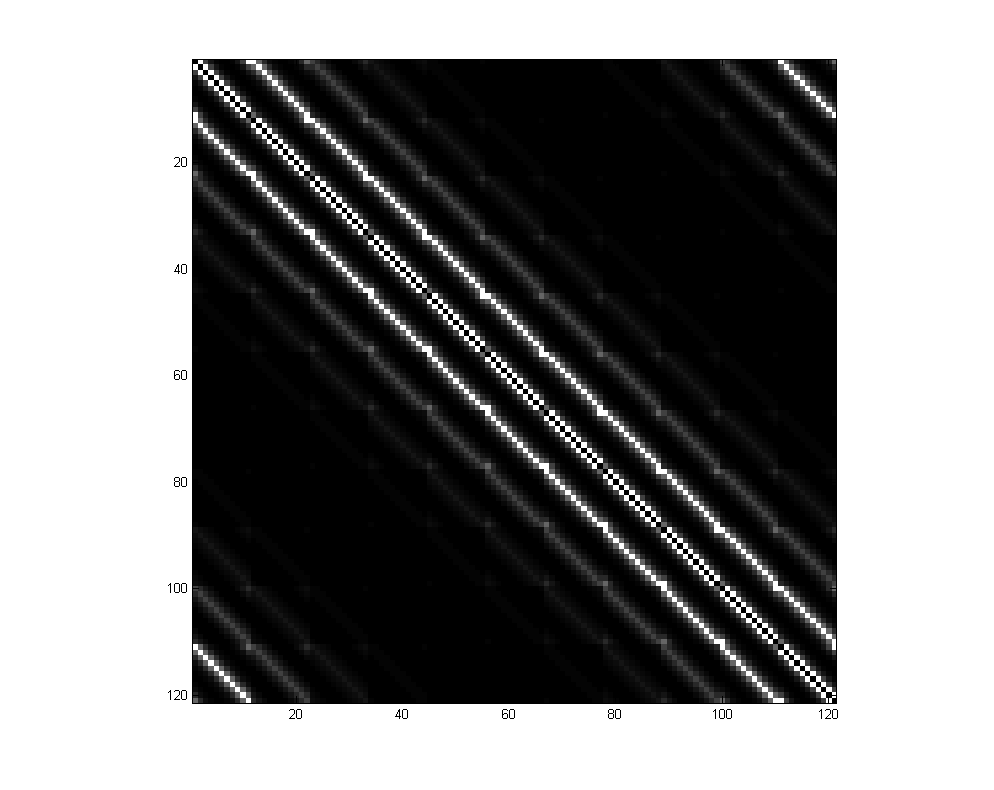
\includegraphics[width=0.9\textwidth]{VMatrixPolicyEvaluation.png}
        
        \caption{	 Colormap of the $V$-values resulting from Policy Evaluation for
        			 $\theta=0$ and $\gamma = 0.8$. \newline
        			 Each axis represents all tiles of the grid world.
        			 The brighter the color the higher the corresponding $V$-value.}  
        \label{colormapPolicyEvaluation}      
\end{figure}


\subsection{Policy Iteration}\label{sec:policyIteration}
Of course the reason for computing the values of all states using Policy Evaluation is to find a good policy. Policy Evaluation gets fed a policy, then computes the values for all states until it converges (i.e. until the largest change in value in one sweep is below $\theta$), and then stops. So after Policy Evaluation we could construct a new policy based on these new values, that would be just as good or better than the policy originally fed to Policy Evaluation. The method of Policy Iteration captures this idea, by repeatedly letting the method of Policy Evaluation be followed by another method called Policy Improvement, until the policy doesn't change anymore. The method of Policy Improvement is explained in Section \ref{policyImprovement}.

\subsubsection{Policy Improvement}\label{policyImprovement}
The idea behind Policy Improvement is that you have determined the value function $V^{\pi}$ for a certain policy $\pi$, and want to know now if any change in the policy could yield a better expected return given this value function. Policy Improvement sweeps through all states to check if any action  $a$ would give a better expected return than the recommended action $\pi(s)$ at that state and if so, $\pi(s) \leftarrow a$. In our stochastic case, this means we need to check for a better probability distribution over the actions at each state, and use the update rule
\begin{equation}
\pi^{k+1}(s) \leftarrow 
			\arg\max_{\pi'(s)} \sum_{a} \pi'(s,a) Q^{\pi^{k}}(s,a)
\end{equation}
Policy Improvement thus yields an improved policy, which can then used to compute the new value function $V$ by Policy Evaluation. This process is repeated by Policy Iteration.


\subsubsection{Results}
The Policy Iteration algorithm has been implemented and run using different settings of $\gamma$. The used values are $\gamma = 0.1$, $\gamma = 0.5$, $\gamma = 0.7$ and $\gamma = 0.9$. 
For each of these runs $\theta$ is set to 0. 
In this report, we provide the $V$-values for the states in which the prey is located at \textbf{(5,5)}. 
The values we found by running Policy Iteration parameterised this way, can be found in Appendix \ref{app:values} in Tables \ref{valueiterationone}, \ref{valueiteration2}, \ref{valueiteration3} and \ref{valueiteration4}. They are exactly the same as those we found with our implementation of Value Iteration (see Section \ref{sec:valueIteration}).

As expected the $V$-values are higher near the goal state, which is \textbf{(5,5)} in this specific case. This will cause the predator to move towards the prey in all cases. Also the values further from the goal state decrease faster in value for lower learning rates. The maximal $V$-value is $10$, which is to be expected with a maximal reward of $10$.



\subsection{Value Iteration}\label{sec:valueIteration}

Value Iteration is another planning algorithm. Just like Policy Iteration (Section \ref{sec:policyIteration}), this algorithm combines the steps of Policy Evaluation and Policy Improvement. However, Value Iteration uses a different approach. Instead of letting Policy Evaluation run until it had converged, Policy Evaluation is stopped after one sweep. In that sweep it combines Policy Evaluation with Policy Improvement in each update step for every state. Its update rule for eahc state is given by Equation \ref{valueIteration}.

\begin{equation}\label{valueIteration}
V_{k+1}(s) \leftarrow \max_a \sum_{s'} \mathcal P_{s s'}^{a} \left( \mathcal R_{s s'}^{a} + \gamma V_{k}(s') \right)
\end{equation}

The algorithm does so by replacing the value of the $(k+1)^{th}$ iteration with the expected reward of the action that maximizes this expectation (based on the $V$-value of $s' $ of the $k^{th}$ iteration and the immediate reward of $s' $), instead of a weighted sum of the expected rewards of all actions. 

\subsubsection{Results}\label{resultsValueIteration}
The Value Iteration algorithm has also been implemented and run using different settings of $\gamma$. The used values are $\gamma = 0.1$, $\gamma = 0.5$, $\gamma = 0.7$ and $\gamma = 0.9$. 
For each of these runs $\theta$ is set to 0. 
In this report, we provide the $V$-values for the states in which the prey is located at \textbf{(5,5)}. 
The results can be found in Appendix \ref{app:values} in Tables \ref{valueiterationone}, \ref{valueiteration2}, \ref{valueiteration3} and \ref{valueiteration4}. These results are exactly the same as those we found with Policy Iteration. 
A representation of the $V$-values which nicely shows the decrease of the $V$-values further from the goal state can be found in Figure \ref{colormapValueIteration}. Here, the symmetry of the state space becomes apparent.

\begin{figure}[htb]
        \center{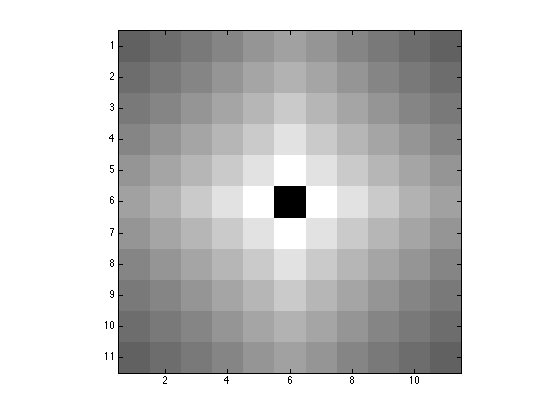
\includegraphics[width=0.7\textwidth]{valueIterationColormap.png}}
        \caption{\label{colormapValueIteration} Colormap of the $V$-values  resulting from Value 
        		Iteration for $\theta=0$ and $\gamma = 0.9$. \newline
        		The brighter the color the higher the corresponding $V$-value.}
\end{figure}

The convergence speed in numbers of iterations is different from those found with Policy Iteration, however. We give an overview in Table \ref{tab:policyEvaluationValues}.

\begin{table}[htb]
\centering
\begin{tabular}{|c|c|c|c|}
\hline 
 & Iterations V.I. & Iterations P.I.  & Total P.E. iterations in P.I. \\ 
\hline 
$\gamma = 0.1 $ & 20 & 8 & 147\\ 
\hline 
$\gamma = 0.5 $ & 28 & 7 & 173\\ 
\hline 
$\gamma = 0.7 $  & 31 & 7 &219 \\ 
\hline 
$\gamma = 0.9 $ & 34 & 8 & 368\\ 
\hline 
\end{tabular}
\caption{Comparison of iterations of Value Iteration and Policy Iteration (P.E. is Policy Evaluation)}
\label{tab:policyEvaluationValues} 
\end{table}

Note that each iteration of Policy Iteration involves a call to Policy Evaluation and Policy Improvement, and both Policy Evaluation and Policy Improvement will sweep through the whole state space. Policy Improvement will do this one time, but Policy Evaluation will often do this multiple times (until the largest change of value is below the threshold $\theta$). Therefore we also kept track of the total numbers of iterations Policy Evaluation had to make in one invocation of Policy Iteration. 

Note, too, that it would be a mistake to compare between the number of iterations for differently parameterised Policy Iteration algorithms. For example, using  $\gamma = 0.1 $ we need the same number of iterations as when using $\gamma = 0.9 $  for convergence, however, comparing the number of times that Policy Evaluation is invoked under these settings, we saw that using the setting of $\gamma = 0.9 $ Policy Iteration had to invoke Policy Evaluation approximately 2.5 times as much as when using the setting of $\gamma = 0.1 $. 

Because each iteration in  Value Iteration sweeps one time through the state space, just like in each iteration in Policy Evaluation, based on the data in Table \ref{tab:policyEvaluationValues} we can reasonably assume that Value Iteration is superior to Policy Iteration in terms of computational complexity when it comes to convergence.




\section{State space reduction}\label{stateSpace}
In the experiments described in Section \ref{simpleStates}, we used a state space that was an intuitive, yet cumbersome representation. We will refer to this state space representation as the ``default'' state space. The amount of states that was used in this default state space was 121 $\times$ 121 = 14641. 

As can be seen in Figure \ref{colormapValueIteration}, there is a symmetry in the state space, and thus relatively much values are redundantly computed.
We elaborated on a more efficient representation for the states, and finally contrived one consisting of $21$ states, an approximately $697$ times smaller one than the default state space. We will refer to this state space representation as the ``efficient'' state space.  By using the symmetry that was present in the state space a much smaller state space was achieved. The expectation is that the computational cost will be lowered, since only 21 state values have to be computed instead of 14641 states. The algorithm has not changed however, so it is also expected that we do not see a large difference in the amount of iterations using the same parameters. 

This efficient state space has been implemented for both Value Iteration and Policy Evaluation. 

Each state represents a distance between the prey and predator. These are represented in the lower left diagonal of a matrix, in which the x-axis is the relative horizontal distance in the MDP and the y-axis the relative vertical distance in the MDP. This matrix is shown in Figure \ref{NewStateRep}. Combinations of positions of prey and predator for which the horizontal and vertical distances are equal are now treated equivalent. 
Also two combinations for which the horizontal distance in one equals the vertical distance in the other and vice versa are considered equal. In order to navigate through this state space different actions are required. These are: \textit{approach horizontal, retreat horizontal, approach vertical, retreat vertical} and as before \textit{wait}. When interacting with the environment these actions are converted into corresponding actions in the real world. This only requires the relative direction of the prey (which is always located at the centre, regardless of its coordinates) with respect to the predator. This is computed by using the difference in location of the prey and predator on the x- and y-axis.

This reduction in the number of states has lead to output values which can be viewed in the appendix section \ref{app:polEvaluation}. The results show that the algorithm does not converge faster in terms of iterations with the efficient state space than with the default state space with $\theta=0$ and $\gamma=0.8$, the default state space required 111 iterations and the efficient state space required 107. 

\begin{figure}[htbp]
        \center{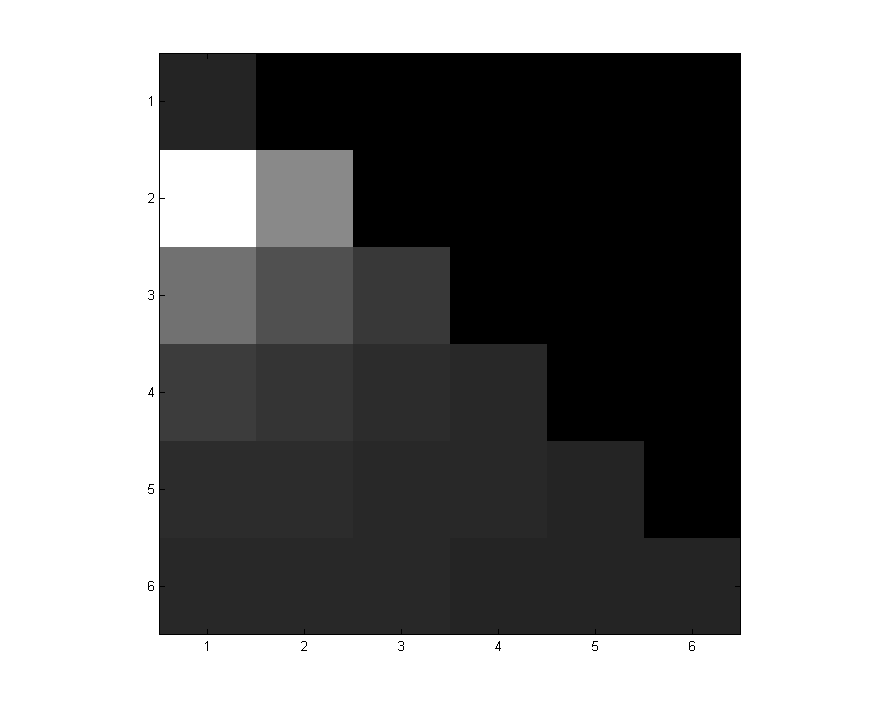
\includegraphics[width=0.6\textwidth]{VMatrixNewStateRep.png}}
        \caption{\label{NewStateRep} Colormap of the $V$-values  resulting from Policy Evaluation for $\theta=0$ and $\gamma = 0.8$ \newline using the ``efficient'' state space representation. The brighter the color the higher the corresponding $V$-value. The prey is always located on the (1, 1) coordinate in this state representation.}
\end{figure}


\section{Conclusion}
We can conclude a few different things.

First, we note that Dynamic Programming (DP) can be deployed successfully for solving reasonably sized MDPs such as the one used throughout this assignment (see Section \ref{environment}). However, a problem using DP methods is that one has to store the values for all states, separately. The number of states grows exponentially with the number of state variables, which can this result in a very large memory use and convergence time. This necessitates one to place much emphasis on contriving an efficient state representation, something which will affect performance very much \cite{sutton} (also see Section \ref{app:classDiagram}) but will be different for every MDP and which will need to be done largely intuitively because no standardized rules or algorithms exist. But this way of state representation also lacks generalisation: if a state is defined by $N$ variables, and the unvisited state $s_1$ is the same as the visited state $s_2$ in $N-1$ variables, using a DP approach state $s_1$ will still have no value at all, despite it being quite similar to $s_2$ for, e.g., $N=10$.

Second, we conclude that Value Iteration appears to be the most efficient converging DP reinforcement learning method for constructing optimal policies compared to Policy Iteration. We refer to Section \ref{resultsValueIteration} for a comparison with Policy Iteration. 


\newpage
\nocite{*}
\bibliographystyle{plainnat}
\bibliography{references}


\newpage
\appendix
\appendixpage
\section{Simulating the Environment} \label{app:firstMust}
Our program's output for the first 100 runs for the random policy predator.\\
\begin{scriptsize}
\begin{verbatim}
	Timesteps:421
	Timesteps:831
	Timesteps:476
	Timesteps:74
	Timesteps:537
	Timesteps:40
	Timesteps:468
	Timesteps:465
	Timesteps:105
	Timesteps:123
	Timesteps:227
	Timesteps:658
	Timesteps:696
	Timesteps:153
	Timesteps:426
	Timesteps:431
	Timesteps:24
	Timesteps:197
	Timesteps:517
	Timesteps:313
	Timesteps:492
	Timesteps:213
	Timesteps:457
	Timesteps:392
	Timesteps:47
	Timesteps:178
	Timesteps:459
	Timesteps:624
	Timesteps:881
	Timesteps:100
	Timesteps:244
	Timesteps:127
	Timesteps:213
	Timesteps:145
	Timesteps:45
	Timesteps:301
	Timesteps:628
	Timesteps:248
	Timesteps:88
	Timesteps:123
	Timesteps:82
	Timesteps:206
	Timesteps:181
	Timesteps:771
	Timesteps:114
	Timesteps:238
	Timesteps:118
	Timesteps:67
	Timesteps:41
	Timesteps:662
	Timesteps:27
	Timesteps:73
	Timesteps:217
	Timesteps:269
	Timesteps:382
	Timesteps:60
	Timesteps:205
	Timesteps:64
	Timesteps:133
	Timesteps:232
	Timesteps:148
	Timesteps:504
	Timesteps:113
	Timesteps:316
	Timesteps:151
	Timesteps:178
	Timesteps:53
	Timesteps:526
	Timesteps:150
	Timesteps:690
	Timesteps:490
	Timesteps:116
	Timesteps:288
	Timesteps:79
	Timesteps:163
	Timesteps:266
	Timesteps:566
	Timesteps:1194
	Timesteps:133
	Timesteps:690
	Timesteps:136
	Timesteps:121
	Timesteps:123
	Timesteps:492
	Timesteps:288
	Timesteps:185
	Timesteps:19
	Timesteps:78
	Timesteps:250
	Timesteps:42
	Timesteps:268
	Timesteps:190
	Timesteps:231
	Timesteps:393
	Timesteps:338
	Timesteps:100
	Timesteps:49
	Timesteps:653
	Timesteps:1173
	Timesteps:421
	Average timesteps over 100 trials: 296.93
	Standard deviation over 100 trials: 244.54689754728025
\end{verbatim}
\end{scriptsize}

\newpage
\section{Policy Iteration and Value Iteration results} \label{app:values}
\subsection*{}
\begin{table}[htbp]
\centering         
                \begin{footnotesize}  
					\begin{tabular} {c c c c c c c c c c c c}
					 & 0 & 1 & 2 & 3 & 4 & 5 & 6 & 7 & 8 & 9 & 10 \\
					0 & 0.000000 & 0.000002 & 0.000011 & 0.000074 & 0.000438 & 0.001730 & 0.000438 & 0.000074 & 0.000011 & 0.000002 & 0.000000\\
					1 & 0.000002 & 0.000011 & 0.000075 & 0.000498 & 0.003195 & 0.013773 & 0.003195 & 0.000498 & 0.000075 & 0.000011 & 0.000002\\
					2& 0.000011 & 0.000075 & 0.000498 & 0.003443 & 0.021739 & 0.117564 & 0.021739 & 0.003443 & 0.000498 & 0.000075 & 0.000011\\
					3 & 0.000074 & 0.000498 & 0.003443 & 0.021739 & 0.166976 & 0.816327 & 0.166976 & 0.021739 & 0.003443 & 0.000498 & 0.000074\\
					4 & 0.000438 & 0.003195 & 0.021739 & 0.166976 & 0.816327 & 10.000000 & 0.816327 & 0.166976 & 0.021739 & 0.003195 & 0.000438\\
					5 & 0.001730 & 0.013773 & 0.117564 & 0.816327 & 10.000000 & 0.000000 & 10.000000 & 0.816327 & 0.117564 & 0.013773 & 0.001730\\
					6 & 0.000438 & 0.003195 & 0.021739 & 0.166976 & 0.816327 & 10.000000 & 0.816327 & 0.166976 & 0.021739 & 0.003195 & 0.000438\\
					7 & 0.000074 & 0.000498 & 0.003443 & 0.021739 & 0.166976 & 0.816327 & 0.166976 & 0.021739 & 0.003443 & 0.000498 & 0.000074\\
					8 & 0.000011 & 0.000075 & 0.000498 & 0.003443 & 0.021739 & 0.117564 & 0.021739 & 0.003443 & 0.000498 & 0.000075 & 0.000011\\
					9 & 0.000002 & 0.000011 & 0.000075 & 0.000498 & 0.003195 & 0.013773 & 0.003195 & 0.000498 & 0.000075 & 0.000011 & 0.000002\\
					10 & 0.000000 & 0.000002 & 0.000011 & 0.000074 & 0.000438 & 0.001730 & 0.000438 & 0.000074 & 0.000011 & 0.000002 & 0.000000\\
					\end{tabular}	
					 \end{footnotesize}				
\caption{The $V$-values for Value Iteration and Policy Iteration, with $\gamma$ = 0.1 and the prey at position \textbf{(5,5)}.}
\label{valueiterationone}
\end{table}

\subsection*{}
\begin{table}[htb]
\centering 
 \begin{footnotesize}  
\begin{tabular} {c c c c c c c c c c c c}
 & 0 & 1 & 2 & 3 & 4 & 5 & 6 & 7 & 8 & 9 & 10 \\
 0 & 0.0267 &  0.0502 &  0.0943 &  0.1768 &  0.3328 &  0.5332 &  0.3328 &  0.1768 &  0.0943 &  0.0502 &  0.0267\\
1 & 0.0502 &  0.0924 &  0.1769 &  0.3390 &  0.6448 &  1.0814 &  0.6448 &  0.3390 &  0.1769 &  0.0924 &  0.0502\\
2 & 0.0943 &  0.1769 &  0.3390 &  0.6498 &  1.2435 &  2.2027 &  1.2435 &  0.6498 &  0.3390 &  0.1769 &  0.0943\\
3 & 0.1768 &  0.3390 &  0.6498 &  1.2435 &  2.3977 &  4.4444 &  2.3977 &  1.2435 &  0.6498 &  0.3390 &  0.1768\\
4 & 0.3328 &  0.6448 &  1.2435 &  2.3977 &  4.4444 & 10.0000 &  4.4444 &  2.3977 &  1.2435 &  0.6448 &  0.3328\\
5 & 0.5332 &  1.0814 &  2.2027 &  4.4444 & 10.0000 &  0.0000 & 10.0000 &  4.4444 &  2.2027 &  1.0814 &  0.5332\\
6 & 0.3328 &  0.6448 &  1.2435 &  2.3977 &  4.4444 & 10.0000 &  4.4444 &  2.3977 &  1.2435 &  0.6448 &  0.3328\\
7 & 0.1768 &  0.3390 &  0.6498 &  1.2435 &  2.3977 &  4.4444 &  2.3977 &  1.2435 &  0.6498 &  0.3390 &  0.1768\\
8 & 0.0943 &  0.1769 &  0.3390 &  0.6498 &  1.2435 &  2.2027 &  1.2435 &  0.6498 &  0.3390 &  0.1769 &  0.0943\\
9 & 0.0502 &  0.0924 &  0.1769 &  0.3390 &  0.6448 &  1.0814 &  0.6448 &  0.3390 &  0.1769 &  0.0924 &  0.0502\\
10 & 0.0267 &  0.0502 &  0.0943 &  0.1768 &  0.3328 &  0.5332 &  0.3328 &  0.1768 &  0.0943 &  0.0502 &  0.0267\\
\end{tabular}\\
\end{footnotesize}
\caption{The $V$-values for Value Iteration and Policy Iteration, with $\gamma$ = 0.5 and the prey at position \textbf{(5,5)}. }
\label{valueiteration2}
\end{table}

\subsection*{}
\begin{table}[htb]
\centering
\begin{footnotesize}
\begin{tabular} {c c c c c c c c c c c c}
 & 0 & 1 & 2 & 3 & 4 & 5 & 6 & 7 & 8 & 9 & 10 \\
0 &  0.4348 &  0.6065 &  0.8453 &  1.1765 &  1.6463 &  2.1169 &  1.6463 &  1.1765 &  0.8453 &  0.6065 &  0.4348\\
1 &  0.6065 &  0.8328 &  1.1750 &  1.6587 &  2.3345 &  3.0759 &  2.3345 &  1.6587 &  1.1750 &  0.8328 &  0.6065\\
2 &  0.8453 &  1.1750 &  1.6587 &  2.3415 &  3.3044 &  4.4805 &  3.3044 &  2.3415 &  1.6587 &  1.1750 &  0.8453\\
3 &  1.1765 &  1.6587 &  2.3415 &  3.3044 &  4.6737 &  6.5116 &  4.6737 &  3.3044 &  2.3415 &  1.6587 &  1.1765\\
4 &  1.6463 &  2.3345 &  3.3044 &  4.6737 &  6.5116 & 10.0000 &  6.5116 &  4.6737 &  3.3044 &  2.3345 &  1.6463\\
5 &  2.1169 &  3.0759 &  4.4805 &  6.5116 & 10.0000 &  0.0000 & 10.0000 &  6.5116 &  4.4805 &  3.0759 &  2.1169\\
6 &  1.6463 &  2.3345 &  3.3044 &  4.6737 &  6.5116 & 10.0000 &  6.5116 &  4.6737 &  3.3044 &  2.3345 &  1.6463\\
7 &  1.1765 &  1.6587 &  2.3415 &  3.3044 &  4.6737 &  6.5116 &  4.6737 &  3.3044 &  2.3415 &  1.6587 &  1.1765\\
8 &  0.8453 &  1.1750 &  1.6587 &  2.3415 &  3.3044 &  4.4805 &  3.3044 &  2.3415 &  1.6587 &  1.1750 &  0.8453\\
9 &  0.6065 &  0.8328 &  1.1750 &  1.6587 &  2.3345 &  3.0759 &  2.3345 &  1.6587 &  1.1750 &  0.8328 &  0.6065\\
10 &  0.4348 &  0.6065 &  0.8453 &  1.1765 &  1.6463 &  2.1169 &  1.6463 &  1.1765 &  0.8453 &  0.6065 &  0.4348\\
\end{tabular}\\
\end{footnotesize}
\caption{The $V$-values for Value Iteration and Policy Iteration, with $\gamma$ = 0.7 and the prey at position \textbf{(5,5)}. }
\label{valueiteration3}
\end{table}

\subsection*{}
\begin{table}[tbp]
\centering
\begin{footnotesize}
\begin{tabular} {c c c c c c c c c c c c}
 & 0 & 1 & 2 & 3 & 4 & 5 & 6 & 7 & 8 & 9 & 10 \\
0 &  3.8831 &  4.2915 &  4.7417 &  5.2374 &  5.7919 &  6.2513 &  5.7919 &  5.2374 &  4.7417 &  4.2915 &  3.8831\\
1 &  4.2915 &  4.7118 &  5.2281 &  5.8024 &  6.4356 &  6.9973 &  6.4356 &  5.8024 &  5.2281 &  4.7118 &  4.2915\\
2 &  4.7417 &  5.2281 &  5.8024 &  6.4401 &  7.1476 &  7.8390 &  7.1476 &  6.4401 &  5.8024 &  5.2281 &  4.7417\\
3 &  5.2374 &  5.8024 &  6.4401 &  7.1476 &  7.9362 &  8.7805 &  7.9362 &  7.1476 &  6.4401 &  5.8024 &  5.2374\\
4 &  5.7919 &  6.4356 &  7.1476 &  7.9362 &  8.7805 & 10.0000 &  8.7805 &  7.9362 &  7.1476 &  6.4356 &  5.7919\\
5 &  6.2513 &  6.9973 &  7.8390 &  8.7805 & 10.0000 &  0.0000 & 10.0000 &  8.7805 &  7.8390 &  6.9973 &  6.2513\\
6 &  5.7919 &  6.4356 &  7.1476 &  7.9362 &  8.7805 & 10.0000 &  8.7805 &  7.9362 &  7.1476 &  6.4356 &  5.7919\\
7 &  5.2374 &  5.8024 &  6.4401 &  7.1476 &  7.9362 &  8.7805 &  7.9362 &  7.1476 &  6.4401 &  5.8024 &  5.2374\\
8 &  4.7417 &  5.2281 &  5.8024 &  6.4401 &  7.1476 &  7.8390 &  7.1476 &  6.4401 &  5.8024 &  5.2281 &  4.7417\\
9 &  4.2915 &  4.7118 &  5.2281 &  5.8024 &  6.4356 &  6.9973 &  6.4356 &  5.8024 &  5.2281 &  4.7118 &  4.2915\\
10 &  3.8831 &  4.2915 &  4.7417 &  5.2374 &  5.7919 &  6.2513 &  5.7919 &  5.2374 &  4.7417 &  4.2915 &  3.8831\\\end{tabular}\\
\end{footnotesize}
\caption{The $V$-values for Value Iteration and Policy Iteration, with $\gamma$ = 0.9 and the prey at position \textbf{(5,5)}.}
\label{valueiteration4}
\end{table}
\FloatBarrier
\subsection*{}

\clearpage
\section{Policy Evaluation comparison}\label{app:polEvaluation}
\subsection{Default state space representation}
Policy Evaluation output with $\theta=0$ and $\gamma$ = 0.8, showing the amount of iterations. This output uses the default state space representation. 
\begin{scriptsize}
\begin{verbatim}
Policy Evaluation, iteration number: 1; maxValueDiff = 2.173444408972901 
Policy Evaluation, iteration number: 2; maxValueDiff = 0.594273911906516 
Policy Evaluation, iteration number: 3; maxValueDiff = 0.288747386234562 
Policy Evaluation, iteration number: 4; maxValueDiff = 0.142434892859105 
Policy Evaluation, iteration number: 5; maxValueDiff = 0.077807292807347 
Policy Evaluation, iteration number: 6; maxValueDiff = 0.043989076413322 
Policy Evaluation, iteration number: 7; maxValueDiff = 0.025523868234365 
Policy Evaluation, iteration number: 8; maxValueDiff = 0.015571413160874 
Policy Evaluation, iteration number: 9; maxValueDiff = 0.009673932990005 
Policy Evaluation, iteration number: 10; maxValueDiff = 0.006050573197382 
Policy Evaluation, iteration number: 11; maxValueDiff = 0.003853977807979 
Policy Evaluation, iteration number: 12; maxValueDiff = 0.002486803847959 
Policy Evaluation, iteration number: 13; maxValueDiff = 0.001609366549420 
Policy Evaluation, iteration number: 14; maxValueDiff = 0.001044912566793 
Policy Evaluation, iteration number: 15; maxValueDiff = 0.000680717843366 
Policy Evaluation, iteration number: 16; maxValueDiff = 0.000452195511078 
Policy Evaluation, iteration number: 17; maxValueDiff = 0.000300871717137 
Policy Evaluation, iteration number: 18; maxValueDiff = 0.000201864159448 
Policy Evaluation, iteration number: 19; maxValueDiff = 0.000136221951843 
Policy Evaluation, iteration number: 20; maxValueDiff = 0.000091909267497 
Policy Evaluation, iteration number: 21; maxValueDiff = 0.000062025880297 
Policy Evaluation, iteration number: 22; maxValueDiff = 0.000042272381132 
Policy Evaluation, iteration number: 23; maxValueDiff = 0.000028863910013 
Policy Evaluation, iteration number: 24; maxValueDiff = 0.000019849447467 
Policy Evaluation, iteration number: 25; maxValueDiff = 0.000013630925504 
Policy Evaluation, iteration number: 26; maxValueDiff = 0.000009359323432 
Policy Evaluation, iteration number: 27; maxValueDiff = 0.000006460531614 
Policy Evaluation, iteration number: 28; maxValueDiff = 0.000004480328471 
Policy Evaluation, iteration number: 29; maxValueDiff = 0.000003102386442 
Policy Evaluation, iteration number: 30; maxValueDiff = 0.000002145040952 
Policy Evaluation, iteration number: 31; maxValueDiff = 0.000001489301996 
Policy Evaluation, iteration number: 32; maxValueDiff = 0.000001035209317 
Policy Evaluation, iteration number: 33; maxValueDiff = 0.000000718422800 
Policy Evaluation, iteration number: 34; maxValueDiff = 0.000000497903405 
Policy Evaluation, iteration number: 35; maxValueDiff = 0.000000344679351 
Policy Evaluation, iteration number: 36; maxValueDiff = 0.000000238380220 
Policy Evaluation, iteration number: 37; maxValueDiff = 0.000000164815624 
Policy Evaluation, iteration number: 38; maxValueDiff = 0.000000114177600 
Policy Evaluation, iteration number: 39; maxValueDiff = 0.000000079027742 
Policy Evaluation, iteration number: 40; maxValueDiff = 0.000000054656798 
Policy Evaluation, iteration number: 41; maxValueDiff = 0.000000037776286 
Policy Evaluation, iteration number: 42; maxValueDiff = 0.000000026094228 
Policy Evaluation, iteration number: 43; maxValueDiff = 0.000000018015862 
Policy Evaluation, iteration number: 44; maxValueDiff = 0.000000012433182 
Policy Evaluation, iteration number: 45; maxValueDiff = 0.000000008577363 
Policy Evaluation, iteration number: 46; maxValueDiff = 0.000000005915533 
Policy Evaluation, iteration number: 47; maxValueDiff = 0.000000004078720 
Policy Evaluation, iteration number: 48; maxValueDiff = 0.000000002811658 
Policy Evaluation, iteration number: 49; maxValueDiff = 0.000000001937877 
Policy Evaluation, iteration number: 50; maxValueDiff = 0.000000001335454 
Policy Evaluation, iteration number: 51; maxValueDiff = 0.000000000920202 
Policy Evaluation, iteration number: 52; maxValueDiff = 0.000000000634014 
Policy Evaluation, iteration number: 53; maxValueDiff = 0.000000000436804 
Policy Evaluation, iteration number: 54; maxValueDiff = 0.000000000300921 
Policy Evaluation, iteration number: 55; maxValueDiff = 0.000000000207302 
Policy Evaluation, iteration number: 56; maxValueDiff = 0.000000000142806 
Policy Evaluation, iteration number: 57; maxValueDiff = 0.000000000098375 
Policy Evaluation, iteration number: 58; maxValueDiff = 0.000000000067767 
Policy Evaluation, iteration number: 59; maxValueDiff = 0.000000000046683 
Policy Evaluation, iteration number: 60; maxValueDiff = 0.000000000032159 
Policy Evaluation, iteration number: 61; maxValueDiff = 0.000000000022154 
Policy Evaluation, iteration number: 62; maxValueDiff = 0.000000000015262 
Policy Evaluation, iteration number: 63; maxValueDiff = 0.000000000010515 
Policy Evaluation, iteration number: 64; maxValueDiff = 0.000000000007244 
Policy Evaluation, iteration number: 65; maxValueDiff = 0.000000000004991 
Policy Evaluation, iteration number: 66; maxValueDiff = 0.000000000003439 
Policy Evaluation, iteration number: 67; maxValueDiff = 0.000000000002369 
Policy Evaluation, iteration number: 68; maxValueDiff = 0.000000000001633 
Policy Evaluation, iteration number: 69; maxValueDiff = 0.000000000001125 
Policy Evaluation, iteration number: 70; maxValueDiff = 0.000000000000775 
Policy Evaluation, iteration number: 71; maxValueDiff = 0.000000000000534 
Policy Evaluation, iteration number: 72; maxValueDiff = 0.000000000000368 
Policy Evaluation, iteration number: 73; maxValueDiff = 0.000000000000254 
Policy Evaluation, iteration number: 74; maxValueDiff = 0.000000000000175 
Policy Evaluation, iteration number: 75; maxValueDiff = 0.000000000000120 
Policy Evaluation, iteration number: 76; maxValueDiff = 0.000000000000083 
Policy Evaluation, iteration number: 77; maxValueDiff = 0.000000000000057 
Policy Evaluation, iteration number: 78; maxValueDiff = 0.000000000000039 
Policy Evaluation, iteration number: 79; maxValueDiff = 0.000000000000027 
Policy Evaluation, iteration number: 80; maxValueDiff = 0.000000000000019 
Policy Evaluation, iteration number: 81; maxValueDiff = 0.000000000000013 
Policy Evaluation, iteration number: 82; maxValueDiff = 0.000000000000009 
Policy Evaluation, iteration number: 83; maxValueDiff = 0.000000000000006 
Policy Evaluation, iteration number: 84; maxValueDiff = 0.000000000000004 
Policy Evaluation, iteration number: 85; maxValueDiff = 0.000000000000003 
Policy Evaluation, iteration number: 86; maxValueDiff = 0.000000000000002 
Policy Evaluation, iteration number: 87; maxValueDiff = 0.000000000000002 
Policy Evaluation, iteration number: 88; maxValueDiff = 0.000000000000001 
Policy Evaluation, iteration number: 89; maxValueDiff = 0.000000000000001 
Policy Evaluation, iteration number: 90; maxValueDiff = 0.000000000000002 
Policy Evaluation, iteration number: 91; maxValueDiff = 0.000000000000001 
Policy Evaluation, iteration number: 92; maxValueDiff = 0.000000000000000 
Policy Evaluation, iteration number: 93; maxValueDiff = 0.000000000000000 
Policy Evaluation, iteration number: 94; maxValueDiff = 0.000000000000000 
Policy Evaluation, iteration number: 95; maxValueDiff = 0.000000000000000 
Policy Evaluation, iteration number: 96; maxValueDiff = 0.000000000000000 
Policy Evaluation, iteration number: 97; maxValueDiff = 0.000000000000000 
Policy Evaluation, iteration number: 98; maxValueDiff = 0.000000000000000 
Policy Evaluation, iteration number: 99; maxValueDiff = 0.000000000000000 
Policy Evaluation, iteration number: 100; maxValueDiff = 0.000000000000000 
Policy Evaluation, iteration number: 101; maxValueDiff = 0.000000000000000 
Policy Evaluation, iteration number: 102; maxValueDiff = 0.000000000000000 
Policy Evaluation, iteration number: 103; maxValueDiff = 0.000000000000000 
Policy Evaluation, iteration number: 104; maxValueDiff = 0.000000000000000 
Policy Evaluation, iteration number: 105; maxValueDiff = 0.000000000000000 
Policy Evaluation, iteration number: 106; maxValueDiff = 0.000000000000000 
Policy Evaluation, iteration number: 107; maxValueDiff = 0.000000000000000 
Policy Evaluation, iteration number: 108; maxValueDiff = 0.000000000000000 
Policy Evaluation, iteration number: 109; maxValueDiff = 0.000000000000000 
Policy Evaluation, iteration number: 110; maxValueDiff = 0.000000000000000 
Policy Evaluation, iteration number: 111; maxValueDiff = 0.000000000000000
\end{verbatim}
\end{scriptsize}
\clearpage
\subsection{Efficient state space representation}
Policy Evaluation output with $\theta=0$ and $\gamma$ = 0.8, showing the amount of iterations. This output uses the efficient state space representation.
\begin{scriptsize}
\begin{verbatim}
Policy Evaluation, iteration number: 1; maxValueDiff = 4.133333333333334 
Policy Evaluation, iteration number: 2; maxValueDiff = 0.979782244071175 
Policy Evaluation, iteration number: 3; maxValueDiff = 0.323017537436372 
Policy Evaluation, iteration number: 4; maxValueDiff = 0.146206941673390 
Policy Evaluation, iteration number: 5; maxValueDiff = 0.074708256161268 
Policy Evaluation, iteration number: 6; maxValueDiff = 0.039836337049262 
Policy Evaluation, iteration number: 7; maxValueDiff = 0.021964360303194 
Policy Evaluation, iteration number: 8; maxValueDiff = 0.012439383912256 
Policy Evaluation, iteration number: 9; maxValueDiff = 0.007203287061450 
Policy Evaluation, iteration number: 10; maxValueDiff = 0.004251480249683 
Policy Evaluation, iteration number: 11; maxValueDiff = 0.002551827008803 
Policy Evaluation, iteration number: 12; maxValueDiff = 0.001562276820132 
Policy Evaluation, iteration number: 13; maxValueDiff = 0.000986274525498 
Policy Evaluation, iteration number: 14; maxValueDiff = 0.000629359330031 
Policy Evaluation, iteration number: 15; maxValueDiff = 0.000405614147592 
Policy Evaluation, iteration number: 16; maxValueDiff = 0.000263813932271 
Policy Evaluation, iteration number: 17; maxValueDiff = 0.000173027918218 
Policy Evaluation, iteration number: 18; maxValueDiff = 0.000114351615488 
Policy Evaluation, iteration number: 19; maxValueDiff = 0.000076586164685 
Policy Evaluation, iteration number: 20; maxValueDiff = 0.000051808453693 
Policy Evaluation, iteration number: 21; maxValueDiff = 0.000035202922172 
Policy Evaluation, iteration number: 22; maxValueDiff = 0.000024014206841 
Policy Evaluation, iteration number: 23; maxValueDiff = 0.000016438856164 
Policy Evaluation, iteration number: 24; maxValueDiff = 0.000011287806742 
Policy Evaluation, iteration number: 25; maxValueDiff = 0.000007771784095 
Policy Evaluation, iteration number: 26; maxValueDiff = 0.000005393725275 
Policy Evaluation, iteration number: 27; maxValueDiff = 0.000003748433468 
Policy Evaluation, iteration number: 28; maxValueDiff = 0.000002608048834 
Policy Evaluation, iteration number: 29; maxValueDiff = 0.000001816438887 
Policy Evaluation, iteration number: 30; maxValueDiff = 0.000001267451277 
Policy Evaluation, iteration number: 31; maxValueDiff = 0.000000886426035 
Policy Evaluation, iteration number: 32; maxValueDiff = 0.000000620141893 
Policy Evaluation, iteration number: 33; maxValueDiff = 0.000000433968556 
Policy Evaluation, iteration number: 34; maxValueDiff = 0.000000303758087 
Policy Evaluation, iteration number: 35; maxValueDiff = 0.000000212659979 
Policy Evaluation, iteration number: 36; maxValueDiff = 0.000000148908623 
Policy Evaluation, iteration number: 37; maxValueDiff = 0.000000104284455 
Policy Evaluation, iteration number: 38; maxValueDiff = 0.000000073042539 
Policy Evaluation, iteration number: 39; maxValueDiff = 0.000000051165928 
Policy Evaluation, iteration number: 40; maxValueDiff = 0.000000035844935 
Policy Evaluation, iteration number: 41; maxValueDiff = 0.000000025113709 
Policy Evaluation, iteration number: 42; maxValueDiff = 0.000000017596447 
Policy Evaluation, iteration number: 43; maxValueDiff = 0.000000012330079 
Policy Evaluation, iteration number: 44; maxValueDiff = 0.000000008640319 
Policy Evaluation, iteration number: 45; maxValueDiff = 0.000000006054990 
Policy Evaluation, iteration number: 46; maxValueDiff = 0.000000004243402 
Policy Evaluation, iteration number: 47; maxValueDiff = 0.000000002973922 
Policy Evaluation, iteration number: 48; maxValueDiff = 0.000000002084287 
Policy Evaluation, iteration number: 49; maxValueDiff = 0.000000001460819 
Policy Evaluation, iteration number: 50; maxValueDiff = 0.000000001023869 
Policy Evaluation, iteration number: 51; maxValueDiff = 0.000000000717630 
Policy Evaluation, iteration number: 52; maxValueDiff = 0.000000000502995 
Policy Evaluation, iteration number: 53; maxValueDiff = 0.000000000352560 
Policy Evaluation, iteration number: 54; maxValueDiff = 0.000000000247119 
Policy Evaluation, iteration number: 55; maxValueDiff = 0.000000000173215 
Policy Evaluation, iteration number: 56; maxValueDiff = 0.000000000121414 
Policy Evaluation, iteration number: 57; maxValueDiff = 0.000000000085105 
Policy Evaluation, iteration number: 58; maxValueDiff = 0.000000000059654 
Policy Evaluation, iteration number: 59; maxValueDiff = 0.000000000041815 
Policy Evaluation, iteration number: 60; maxValueDiff = 0.000000000029311 
Policy Evaluation, iteration number: 61; maxValueDiff = 0.000000000020546 
Policy Evaluation, iteration number: 62; maxValueDiff = 0.000000000014402 
Policy Evaluation, iteration number: 63; maxValueDiff = 0.000000000010095 
Policy Evaluation, iteration number: 64; maxValueDiff = 0.000000000007076 
Policy Evaluation, iteration number: 65; maxValueDiff = 0.000000000004960 
Policy Evaluation, iteration number: 66; maxValueDiff = 0.000000000003477 
Policy Evaluation, iteration number: 67; maxValueDiff = 0.000000000002437 
Policy Evaluation, iteration number: 68; maxValueDiff = 0.000000000001709 
Policy Evaluation, iteration number: 69; maxValueDiff = 0.000000000001198 
Policy Evaluation, iteration number: 70; maxValueDiff = 0.000000000000839 
Policy Evaluation, iteration number: 71; maxValueDiff = 0.000000000000588 
Policy Evaluation, iteration number: 72; maxValueDiff = 0.000000000000412 
Policy Evaluation, iteration number: 73; maxValueDiff = 0.000000000000289 
Policy Evaluation, iteration number: 74; maxValueDiff = 0.000000000000203 
Policy Evaluation, iteration number: 75; maxValueDiff = 0.000000000000142 
Policy Evaluation, iteration number: 76; maxValueDiff = 0.000000000000100 
Policy Evaluation, iteration number: 77; maxValueDiff = 0.000000000000070 
Policy Evaluation, iteration number: 78; maxValueDiff = 0.000000000000049 
Policy Evaluation, iteration number: 79; maxValueDiff = 0.000000000000034 
Policy Evaluation, iteration number: 80; maxValueDiff = 0.000000000000024 
Policy Evaluation, iteration number: 81; maxValueDiff = 0.000000000000017 
Policy Evaluation, iteration number: 82; maxValueDiff = 0.000000000000012 
Policy Evaluation, iteration number: 83; maxValueDiff = 0.000000000000008 
Policy Evaluation, iteration number: 84; maxValueDiff = 0.000000000000006 
Policy Evaluation, iteration number: 85; maxValueDiff = 0.000000000000004 
Policy Evaluation, iteration number: 86; maxValueDiff = 0.000000000000003 
Policy Evaluation, iteration number: 87; maxValueDiff = 0.000000000000002 
Policy Evaluation, iteration number: 88; maxValueDiff = 0.000000000000001 
Policy Evaluation, iteration number: 89; maxValueDiff = 0.000000000000001 
Policy Evaluation, iteration number: 90; maxValueDiff = 0.000000000000001 
Policy Evaluation, iteration number: 91; maxValueDiff = 0.000000000000000 
Policy Evaluation, iteration number: 92; maxValueDiff = 0.000000000000000 
Policy Evaluation, iteration number: 93; maxValueDiff = 0.000000000000000 
Policy Evaluation, iteration number: 94; maxValueDiff = 0.000000000000000 
Policy Evaluation, iteration number: 95; maxValueDiff = 0.000000000000001 
Policy Evaluation, iteration number: 96; maxValueDiff = 0.000000000000000 
Policy Evaluation, iteration number: 97; maxValueDiff = 0.000000000000000 
Policy Evaluation, iteration number: 98; maxValueDiff = 0.000000000000000 
Policy Evaluation, iteration number: 99; maxValueDiff = 0.000000000000000 
Policy Evaluation, iteration number: 100; maxValueDiff = 0.000000000000000 
Policy Evaluation, iteration number: 101; maxValueDiff = 0.000000000000000 
Policy Evaluation, iteration number: 102; maxValueDiff = 0.000000000000000 
Policy Evaluation, iteration number: 103; maxValueDiff = 0.000000000000000 
Policy Evaluation, iteration number: 104; maxValueDiff = 0.000000000000000 
Policy Evaluation, iteration number: 105; maxValueDiff = 0.000000000000000 
Policy Evaluation, iteration number: 106; maxValueDiff = 0.000000000000000 
Policy Evaluation, iteration number: 107; maxValueDiff = 0.000000000000000
\end{verbatim}
\end{scriptsize} 

\section*{}
\clearpage
\section{Class diagram}\label{app:classDiagram}
\begin{figure}[htb]
        \center{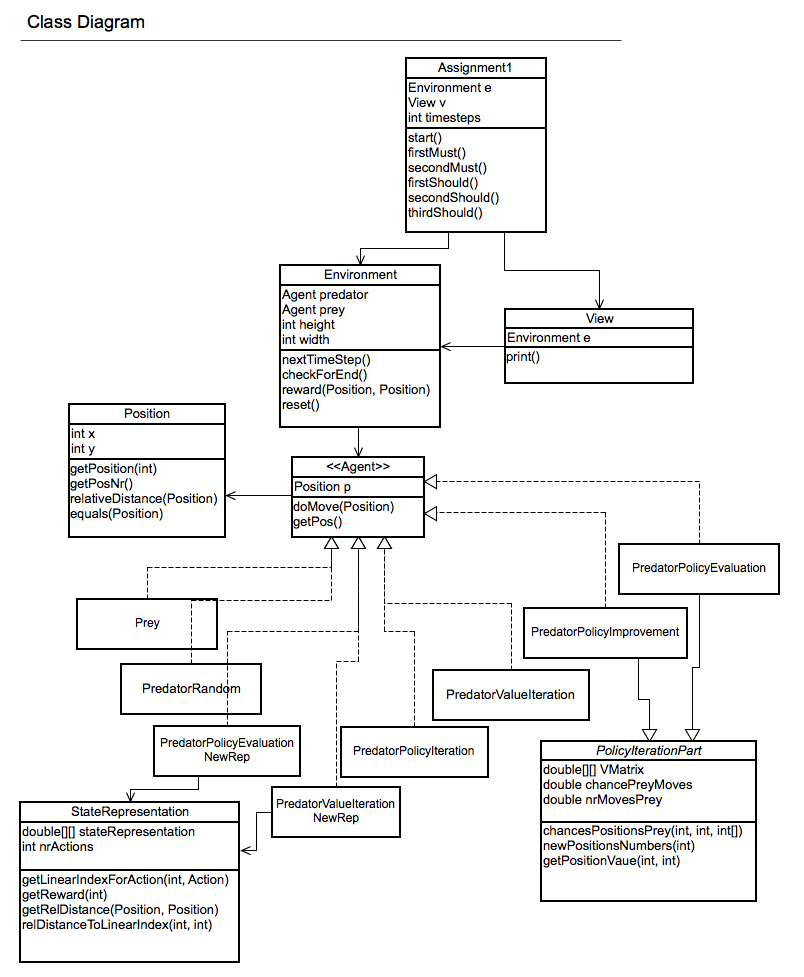
\includegraphics[width=0.82\textwidth]{classDiagram.png}}
        \caption{\label{pic:classDiagram} A class diagram of our code. For clarity purposes, not all methods and attributes of the classes are shown.}
\end{figure}



%\end{landscape}



\end{document}
